\documentclass[tikz,border=2pt]{standalone}
\usepackage{amsmath}
\usepackage{pgfplots}
\pgfplotsset{compat=1.18}

\begin{document}
% Critical points: where f'(x)=0 (horizontal tangent) or where f' does not exist (a corner).
% Left: f(x)=x^3-3x+1 has f'=0 at x=-1 and x=1. Right: g(x)=|x-3.5|+1 has no derivative at 3.5.
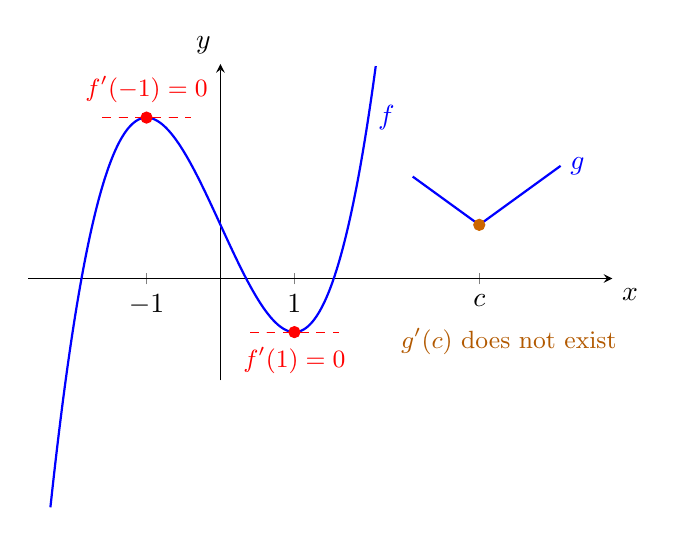
\begin{tikzpicture}
	\begin{axis}[
		axis lines=middle,
		xmin=-2.6, xmax=5.3,
		ymin=-1.9, ymax=4.0,
		xtick={-1,1,3.5}, xticklabels={$-1$,$1$,$c$},
		ytick=\empty,
		xlabel={$x$}, ylabel={$y$},
		xlabel style={below right}, ylabel style={above left},
		samples=150, smooth, clip=false,
		width=9cm, height=5.6cm
		]
		\addplot[thick, blue, domain=-2.3:2.1] {x^3-3*x+1};
		\addplot[red, dashed, domain=-1.6:-0.4] {3};
		\addplot[red, dashed, domain=0.4:1.6] {-1};
		\addplot[only marks, mark=*, red] coordinates {(-1,3) (1,-1)};
		\node[red, anchor=south, font=\small] at (axis cs:-1,3.1) {$f'(-1)=0$};
		\node[red, anchor=north, font=\small] at (axis cs:1,-1.1) {$f'(1)=0$};
		\addplot[thick, blue, domain=2.6:3.5, samples=2] {-(x-3.5)+1};
		\addplot[thick, blue, domain=3.5:4.6, samples=2] {(x-3.5)+1};
		\addplot[only marks, mark=*, orange!80!black] coordinates {(3.5,1)};
		\node[orange!70!black, anchor=north, font=\small] at (axis cs:3.9,-0.75) {$g'(c)$ does not exist};
		\node[blue, anchor=west] at (axis cs:2.0,3.0) {$f$};
		\node[blue, anchor=west] at (axis cs:4.6,2.1) {$g$};
	\end{axis}
\end{tikzpicture}
\end{document}
